\documentclass{article}

\usepackage[utf8]{inputenc}
\usepackage[spanish]{babel} % Configura el idioma en español
\usepackage{titlesec}
\usepackage{titling}
\usepackage{lipsum}
\usepackage{graphicx}
\usepackage{xcolor}
\usepackage{float}
\usepackage[left=2cm, right=2cm, top=2cm, bottom=2cm]{geometry}

\title{App participación ciudadana - Informe técnico}
\author{Nicolás García Sastre}
\date{\today}

\begin{document}
 
\begin{titlepage}
    \centering
    
\includegraphics[width=0.6\textwidth]{logos/LOGOAZALEA.png}\par\vspace{1cm}
    \begin{flushright}
        {\Large\bfseries\thetitle\par}
        \rule{1\textwidth}{1pt}\par
        {\color{gray}\Large\theauthor\par}
    \end{flushright}
    \vfill
    {\large\thedate\par}
\end{titlepage}

\tableofcontents

\newpage

\section{Tarea}

\subsection{Objetivo perseguido}
Existe una necesidad imperante de abordar los desafíos y motores socio-psicológicos, socio-técnicos e institucionales que impactan la participación efectiva del público en proyectos de infraestructura energética y urbana. Nuestra meta es explorar estrategias para superar las barreras existentes y lograr una participación significativa dentro de la comunidad universitaria. 

Algunos problemas frecuentes en proyectos de participación ciudadana incluyen la falta de conexión entre el proyecto y las necesidades/intereses ciudadanos, lo que resulta en baja participación. Además, si los resultados no se traducen en acciones concretas o las expectativas no se cumplen, los ciudadanos pueden volverse desilusionados y menos propensos a participar en el futuro. La falta de incentivos tangibles o reconocimiento también puede disminuir el interés ciudadano.

En este contexto, surge la necesidad de proponer la creación de una aplicación web de participación ciudadana ``Azalea - Participa''. Esta iniciativa busca fortalecer la relación entre la comunidad y el tejido urbano, construyendo confianza y apoyo. La aplicación generará un mapa interactivo que recogerá no solo rutas habituales, áreas sin vegetación, zonas y espacios en mal estado, sino también las preocupaciones y sugerencias puntuales de la comunidad, a través de anotaciones digitales geolocalizadas que hará cada usuario desde su mapa. Tras un periodo de tiempo, las anotaciones individuales de cada usuario se recopilarán en el mismo plano, facilitando una percepción visual de los problemas y sugerencias más reportados, además de proporcionar una base de datos completa sobre la percepción de la comunidad universitaria, que usará nuestro equipo para desarrollar soluciones en el campus de Vera.

\subsection{Descripción del trabajo realizado}

Durante el desarrollo de la aplicación ``Azalea - Participa'', nos enfocamos en crear una plataforma interactiva que fomente la participación ciudadana en proyectos de infraestructura. Implementamos un mapa interactivo que permite a los usuarios abrir, comentar y respaldar incidencias en tiempo real. Hemos diseñado la interfaz de manera intuitiva para facilitar la geolocalización de problemas urbanos y recopilamos estas anotaciones para proporcionar una visión visual y detallada de las preocupaciones de la comunidad universitaria.

\newpage

\section{Trabajo realizado}



\subsection{Casos de uso}

Los casos de uso son una herramienta fundamental en el desarrollo de software que permite definir, describir y comprender las interacciones entre los usuarios y un sistema o aplicación. Consisten en representaciones narrativas de cómo los usuarios interactúan con el sistema para lograr objetivos específicos. Estas representaciones proporcionan una visión clara y detallada de los requisitos funcionales de la aplicación, delineando las diversas acciones que los usuarios pueden llevar a cabo y cómo el sistema responde a estas acciones.

Los casos de uso delineados en este informe abarcan una amplia gama de interacciones entre los usuarios y la aplicación, desde la creación y el seguimiento de incidencias hasta la gestión y resolución por parte de los moderadores. Cada caso de uso está diseñado para optimizar la experiencia del usuario, garantizando una navegación intuitiva y una interacción fluida con la plataforma.

Se han realizado tres casos de uso, dividiéndolos en tipos de usuario.

\begin{figure}[H]
    \center
    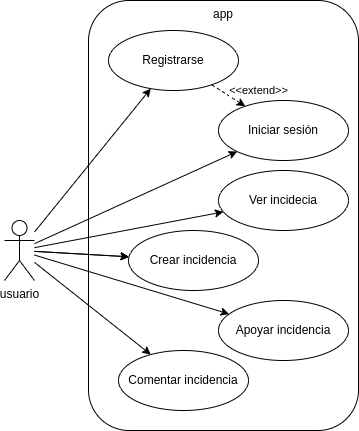
\includegraphics[width=6cm]{images/caso_de_uso_usuario.png}
    \caption{Casos de uso de usuario.}
    \label{fig:caso_uso_usuario}
\end{figure}


En la figura \ref{fig:caso_uso_usuario}, se presentan los casos de uso destinados al usuario de la aplicación, delineando las diversas interacciones que este puede llevar a cabo. Estos casos de uso son esenciales para comprender cómo el usuario interactúa con el sistema y qué funcionalidades están disponibles para él.

El usuario de la aplicación cuenta con una serie de acciones a su disposición, las cuales se detallan a continuación:

\begin{itemize}
    \item \textbf{Visualización de incidencias:} Este caso de uso permite al usuario explorar y visualizar las incidencias reportadas en el mapa. A través de esta funcionalidad, el usuario puede obtener información relevante sobre problemas o situaciones que requieren atención en ubicaciones específicas.

    \item \textbf{Registro e inicio de sesión:} En este caso de uso, el usuario tiene la opción de registrarse en la plataforma para acceder a funcionalidades adicionales o iniciar sesión si ya cuenta con una cuenta previamente creada. El registro y el inicio de sesión son pasos fundamentales para garantizar la seguridad y la personalización de la experiencia del usuario.
    
    \item \textbf{Creación de incidencias:} Mediante este caso de uso, el usuario puede reportar nuevas incidencias al sistema. Esto implica proporcionar detalles sobre la naturaleza del problema, adjuntar imágenes u otros archivos relevantes, y asignar una ubicación geográfica precisa para facilitar su posterior gestión y resolución.
    
    \item \textbf{Apoyo a incidencias:} Aquí, el usuario tiene la capacidad de expresar su apoyo o solidaridad hacia una incidencia específica. Esta función fomenta la participación y la colaboración entre los usuarios, permitiéndoles mostrar su interés y preocupación por determinadas situaciones.
    
    \item \textbf{Comentarios en incidencias:} Este caso de uso habilita al usuario para agregar comentarios adicionales a una incidencia existente. A través de esta funcionalidad, los usuarios pueden proporcionar información adicional, sugerir soluciones o simplemente expresar sus opiniones sobre un problema en particular, fomentando así la interacción y el intercambio de ideas dentro de la comunidad.
\end{itemize}

\begin{figure}[H]
    \center
    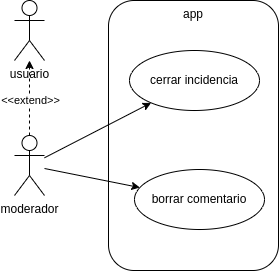
\includegraphics[width=5cm]{images/caso_de_uso_moderador.png}
    \caption{Casos de uso de moderador.}
    \label{fig:caso_uso_mod}
\end{figure}

En la figura \ref{fig:caso_uso_mod}, se exhiben los casos de uso concebidos para los moderadores de la aplicación, detallando las funciones y responsabilidades específicas que tienen dentro del sistema. Estos casos de uso son detallan cómo los moderadores interactúan con la plataforma y cómo ejercen su rol de supervisión y gestión de contenidos.

Los casos de uso destinados a los moderadores incluyen:

\begin{itemize}
    \item \textbf{Cierre de incidencias:} Este caso de uso permite al moderador finalizar o cerrar incidencias una vez que han sido debidamente atendidas o resueltas. Al cerrar una incidencia, el moderador indica que se han tomado las medidas necesarias para abordar el problema reportado, proporcionando así un seguimiento completo del ciclo de vida de la incidencia. También puede cerrar incidencias debido a que han sido indebidamente reportadas.
    
    \item \textbf{Borrado de comentarios:} En este caso de uso, el moderador tiene la capacidad de eliminar comentarios inapropiados, ofensivos o irrelevantes que hayan sido publicados en las incidencias. Esta función garantiza que el contenido dentro de la plataforma se mantenga adecuado y respetuoso, promoviendo un entorno de colaboración y participación positiva entre los usuarios.
\end{itemize}

\begin{figure}[H]
    \center
    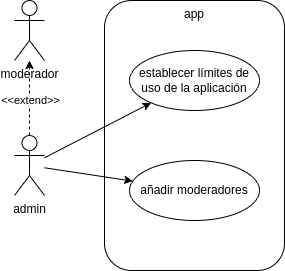
\includegraphics[width=5cm]{images/caso_de_uso_admin.png}
    \caption{Casos de uso de administrador.}
    \label{fig:caso_uso_admin}
\end{figure}

En la figura \ref{fig:caso_uso_admin}, se presentan los casos de uso diseñados específicamente para los administradores de la aplicación. Estos usuarios poseen privilegios adicionales que les permiten gestionar aspectos críticos del sistema y asegurar su correcto funcionamiento.

Los casos de uso para los administradores incluyen:
\begin{itemize}
    \item \textbf{Establecimiento de límites geográficos:} Este caso de uso otorga al administrador la capacidad de definir y modificar los límites geográficos dentro de los cuales la aplicación estará disponible para su uso. Esto puede incluir la delimitación de áreas específicas de servicio o la restricción de la aplicación a ciertos territorios, adaptando así la aplicación a las necesidades y requisitos particulares de cada contexto.
    \item \textbf{Adición de usuarios moderadores:} En este caso de uso, el administrador puede agregar nuevos usuarios al rol de moderador, otorgándoles así permisos y responsabilidades adicionales dentro del sistema. La capacidad de añadir moderadores es crucial para distribuir la carga de trabajo y garantizar una supervisión efectiva de las incidencias y los comentarios en la plataforma.
\end{itemize}

\subsection{Desarrollo}

Para este proyecto, desde control, se contaba con unos prototipos ya realizados en formato PDF (figura \ref{fig:prototipos-previos}). Dados estos prototipos, se ha utilizado React para implementar la interfaz de la aplicación en formato web. Aunque ya se tenían prototipos, se han tenido que desarrollar otras vistas que no estaban prototipadas, como podrían ser la vista del login, o la vista para añadir una incidencia (fogira \ref{fig:prototipos-creados}). Desde el primer momento se ha tratado que dicha web sea usable tanto en dispositivos móbiles cómo en ordenadores. Para la parte del backend, se ha utilizado python junto con flask. 

La aplicación ha sido estructurada de manera que el frontend y el backend funcionen como servicios separados. Esto significa que cada uno puede ser ejecutado en máquinas o entornos en la nube diferentes. En lugar de tener ambos componentes acoplados de manera inseparable, la arquitectura de la aplicación permite una mayor flexibilidad al permitir que el frontend y el backend operen de manera independiente.

\begin{figure}[H]
    \center
    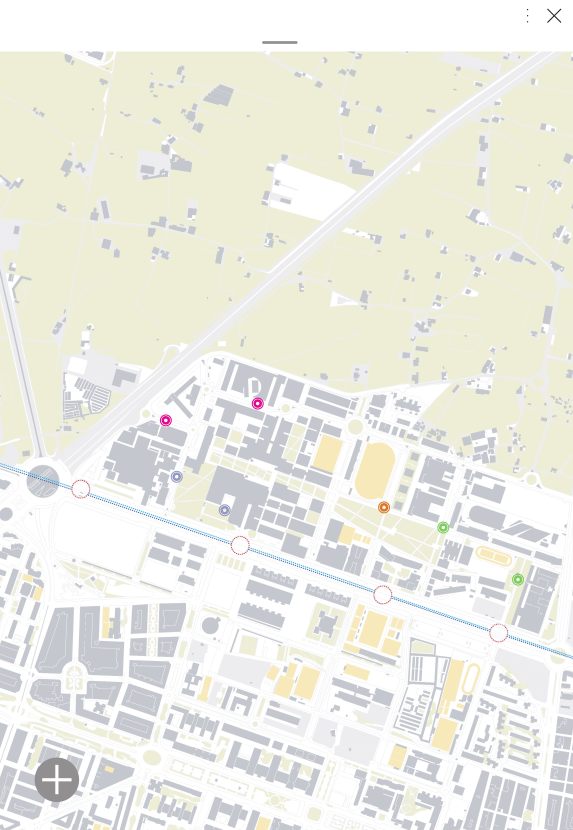
\includegraphics[width=6cm]{images/mockup1.png}
    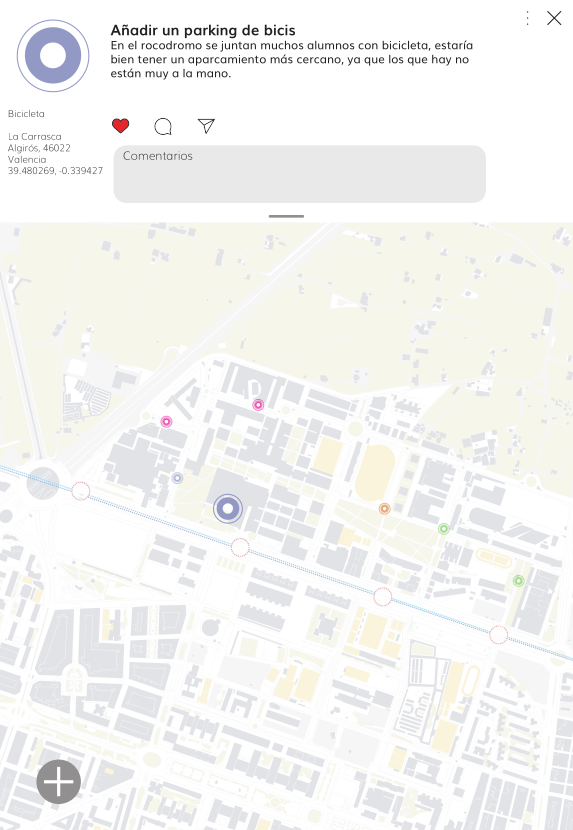
\includegraphics[width=6cm]{images/mockup2.png}
    \caption{Prototipos previos al desarrollo.}
    \label{fig:prototipos-previos}
\end{figure}

\begin{figure}[H]
    \center
    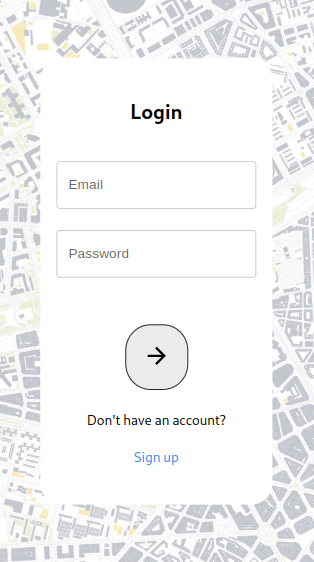
\includegraphics[width=6cm]{images/login.png}
    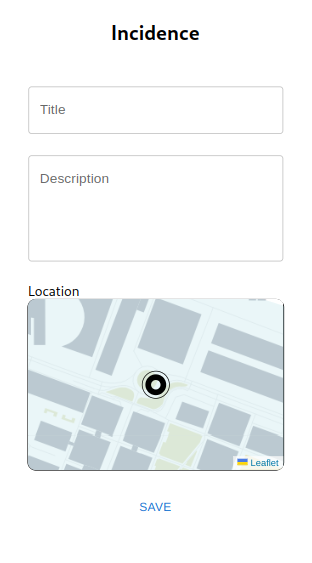
\includegraphics[width=6cm]{images/crear_incidencia.png}
    \caption{Prototipos creados para el desarrollo.}
    \label{fig:prototipos-creados}
\end{figure}

\subsubsection{Obtención de mapas para la aplicación}

El primer paso en el desarrollo de la aplicación fue la obtención de un mapa personalizado. Dado que los prototipos incluían mapas personalizados, se buscó una herramienta para la visualización de mapas en el frontend que permitiera la integración de mapas personalizados. Esta herramienta seleccionada fue Leaflet. Leaflet permite la incorporación de una URL personalizada para obtener los "Tiles" (teselas) que componen el mapa visible en pantalla.

En el contexto de Leaflet, los "Tiles" son imágenes cuadradas pequeñas que forman el mosaico visible del mapa. Estas imágenes son descargadas dinámicamente a medida que el usuario navega por el mapa. La utilización de "Tiles" facilita la visualización eficiente de mapas personalizados, ya que solo se descargan las partes necesarias, optimizando así la carga y la velocidad de respuesta de la aplicación. 

La obtención, tanto de los mapas como de los tiles, se realizó utilizando la herramienta QGIS. QGIS es un sistema de información geográfica (SIG) de código abierto que ofrece funcionalidades robustas para la visualización, análisis y procesamiento de datos geoespaciales.

\begin{figure}[H]
    \center
    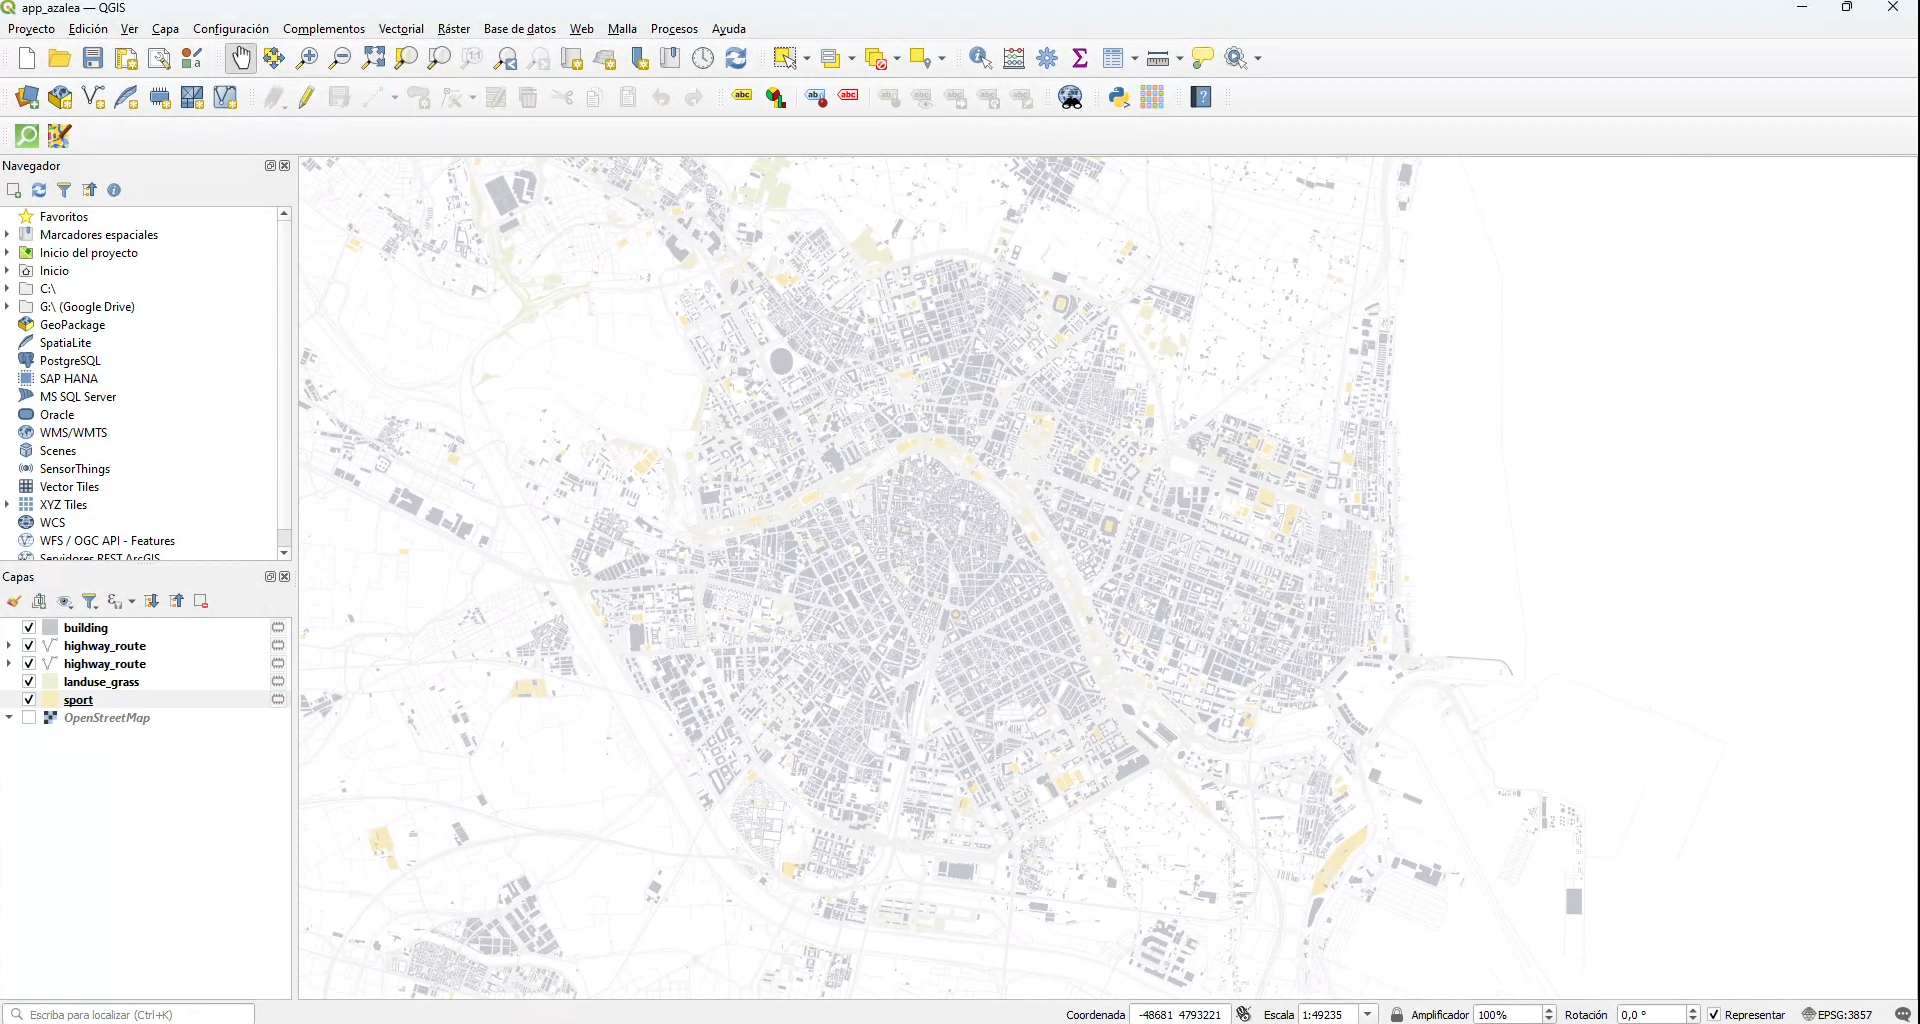
\includegraphics[width=14cm]{images/qgis.png}
    \caption{QGIS}
    \label{fig:qgis}
\end{figure}

Con QGIS y el plugin QuickOSM se obtuvieron las capas necesarias para la aplicación. Posteriormente, se editaron los colores de cada una de las capas, tal y como se muestra en la figura \ref{fig:qgis}. Finalmente, se utilizó el plugin QTiles para la renderización de los tiles para la aplicación.

\subsubsection{Desarrollo del frontend}

Para el desarrollo del frontend, se han considerado las distintas vistas representadas en el diagrama de navegación del usuario, como se muestra en la figura \ref{fig:diagrama_navegacion_usuario}.

\begin{figure}[H]
\centering
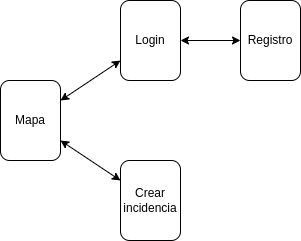
\includegraphics[width=5cm]{images/diagrama_vistas.png}
\caption{Diagrama de la navegación del usuario entre las vistas de la aplicación.}
\label{fig:diagrama_navegacion_usuario}
\end{figure}

Las vistas contempladas son las siguientes:

\begin{itemize}
    \item \textbf{Mapa:} Esta vista es la vista principal de la aplicación. Proporciona al usuario una representación visual de las incidencias reportadas en un mapa geográfico. Aquí, los usuarios pueden explorar las ubicaciones de las incidencias y acceder a detalles adicionales (como la descripción, comentarios o número de apoyos) haciendo click sobre ellas. 
    \item \textbf{Login:} La vista de inicio de sesión permite a los usuarios autenticarse en la aplicación, proporcionando credenciales válidas, como nombre de usuario y contraseña, para acceder a funcionalidades exclusivas y personalizadas.
    \item \textbf{Registro:} En esta vista, los usuarios tienen la posibilidad de crear una nueva cuenta en la aplicación proporcionando la información requerida, como nombre, dirección de correo electrónico y contraseña. El registro es necesario para acceder a determinadas funcionalidades y para establecer una identidad única en la plataforma.
    \item \textbf{Crear incidencia:} Esta vista permite a los usuarios reportar nuevas incidencias en el sistema. Aquí, los usuarios pueden proporcionar detalles sobre el problema observado y especificar la ubicación geográfica exacta de la incidencia mediante un mapa interactivo.
\end{itemize}

Además de estas vistas, existe una vista adicional de \textbf{configuración}, en la que los usuarios administradores pueden establecer los límites geográficos del uso de la aplicación y gestionar los usuarios moderadores.

\subsubsection{Desarrollo del backend}

\newpage

\section{Conclusiones}

\end{document}